
\chapter{Results}


\todo{Today, I changed the test criterion from the output neuron voltage at time $t$ to a mean over a sample of the last
    $20ms$, network performance improved tremendously. Intuitively makes sense, but in particular it makes NEST networks
    diverge less after peak performance is reached. Are fluctuations in output layer activity increasing during late
    stages of training?}

\todo{it might be worth experimenting with different synaptic delays in NEST in order to evaluate learning performance
    under biologically plausible transmission times. How easy this will \textbf{assumably} be to implement in NEST
    deserves note at this point.}

\todo{talk about the fact that NEST synapses are updated, and SpikeEvents stored to ring buffers to be integrated into
    $u_som$ after the synaptic delay. How much of physiological synaptic delays occurs pre- and postsynaptically in
    pyramidal neurons?}

\section{direct feedback connections to interneurons}\label{sec-electric-syns}

\cite{Vaughn2022,Mancilla2007}


\section{The self-predicting state}

As a first comparison between the three implmementations, the pre-training towards a self-predicting stat (cf.
\cite{sacramento2018dendritic} Figure S1) was performed with equal parametrizations, as shown in Figure
\ref{fig-self-pred}. For this experiment, no target signal was provided at the output layer, and the network was
stimulated with random inputs.



\begin{figure}[t]
    \centering
    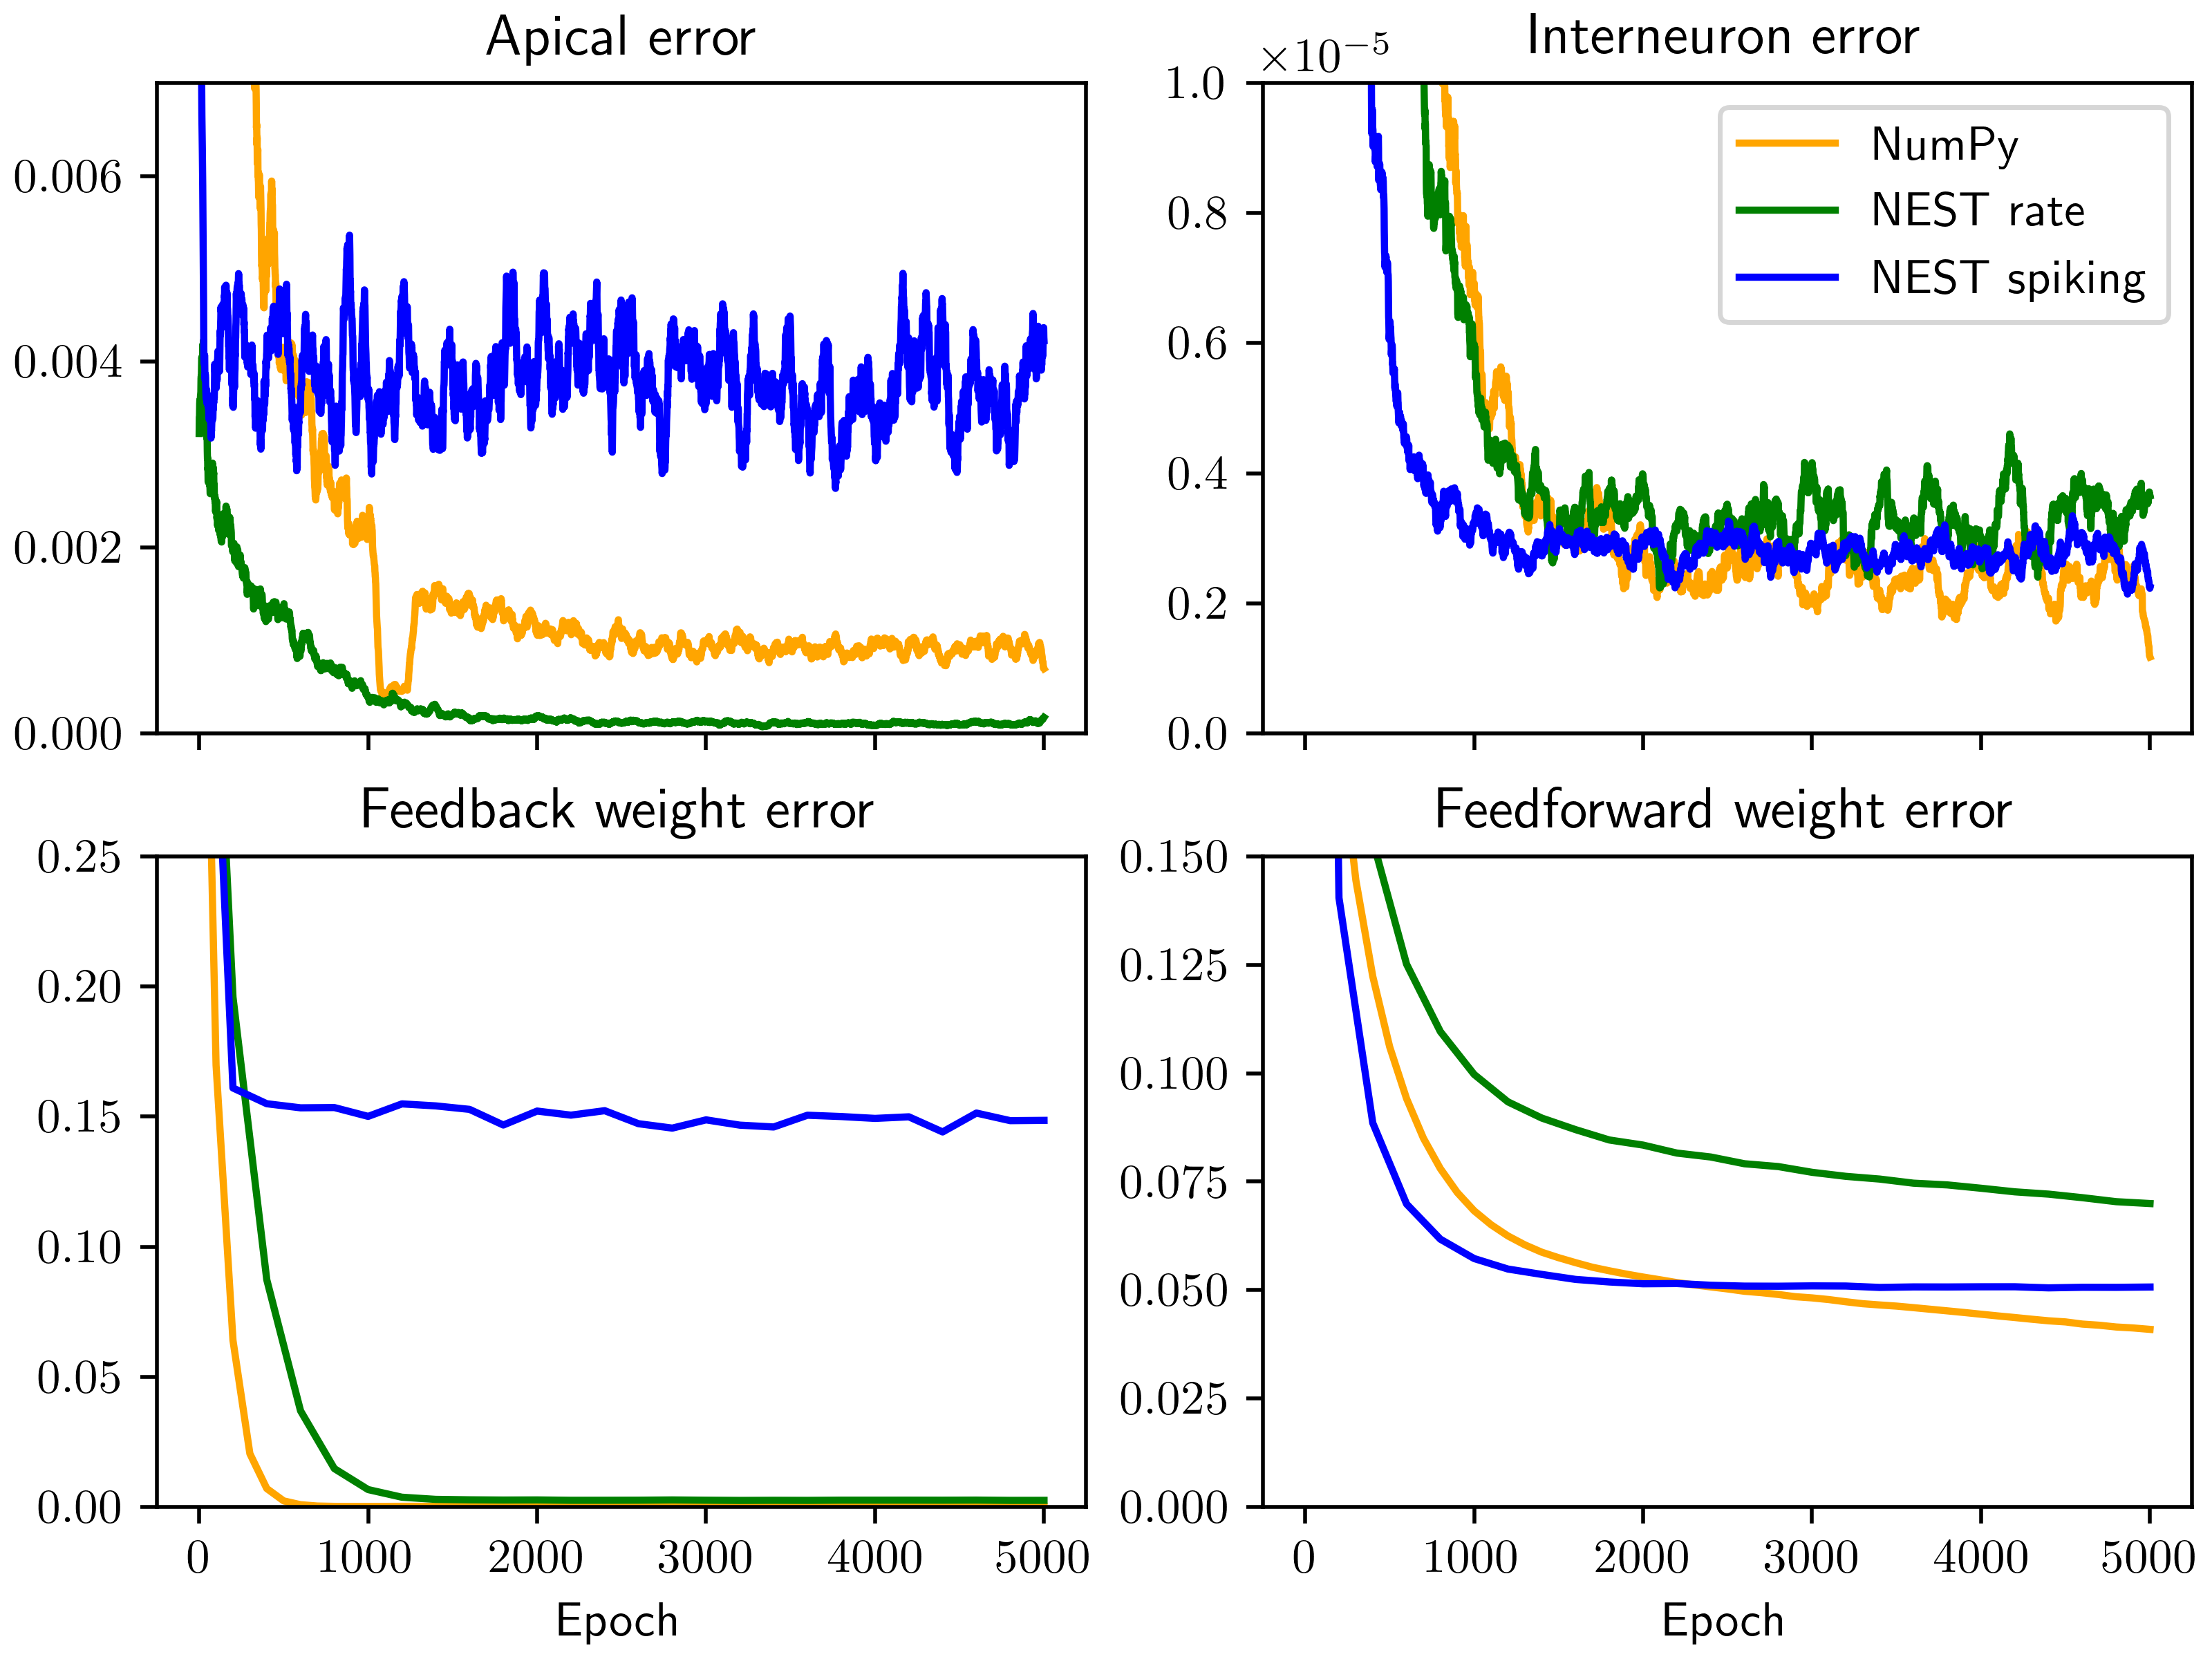
\includegraphics[width=0.9\textwidth]{fig_self_prediction}
    \caption{Different network types learn to predict self-generated activity in superficial layers. All networks were
        initialized with dimensions $[6, 10, 3]$, and stimulated with $5000$ samples of random input for $100ms$ each.
        As described in \cite{sacramento2018dendritic}, during only Pyramidal-Interneuron and Interneuron-Pyramidal
        weights are plastic ($\eta^{pi}=0.05, \eta^{ip}=0.02375, \eta^{up}=\eta^{down}=0$). All variants reach a
        self-predicting state within the first 1000 stimulus presentations and errors remain stable after that point.}
    \label{fig-self-pred}
\end{figure}

All implementations were able to reach comparable values for the four error metrics after roughly the same time. The
exact values that errors converge on differs slightly between implementations, but generally is on the same order of
magnitude and thus does not hinder learning performance greatly (cf. Section \ref{sec-le-tpres}). A notable outlier is
the apical error of pyramidal neuron in the spike-based implementation. This can however be traced back to individual
spikes causing substantial deviations in apical potentials, and can therefore be alleviated by increasing the
\textit{weight\_scale} parameter (results not shown) at the cost of increased training time. Alternatively, increasing
the membrane capacitance of the apical compartment also solves the issue as it smoothes out the effect of individual
spikes. Yet this solution also increases the relaxation period of the entire network, requiring a highly
undesirable increase in $t_{pres}$ for successful learning. Since weight errors converge to similar values as the
rate-based implementations, an increased absolute apical compartment voltage was deemed tolerable.

\section{Delayed presentation of instructive signals}

A key concern of biologically plausible learning is the issue of when an instructive signal becomes available for
training the network \todo{cite or nah?}. When an organism is presented with a stimulus that requires a specific action,
the organism responds to the best of its ability. Yet, the consequences of that response are likely to be delayed.
\todo{do we want this section?}


\section{Presentation times with latent equilibrium}\label{sec-le-tpres}

In order to validate the performance of my implementations, I replicated a parameter study from \cite{Haider2021}[Fig.
    3]. The results for the NEST network using spiking neurons with default parameters \todo{elaborate on this} are
shown in Figure \ref{fig-bars-le-snest}. A



\begin{figure}[t]
    \centering
    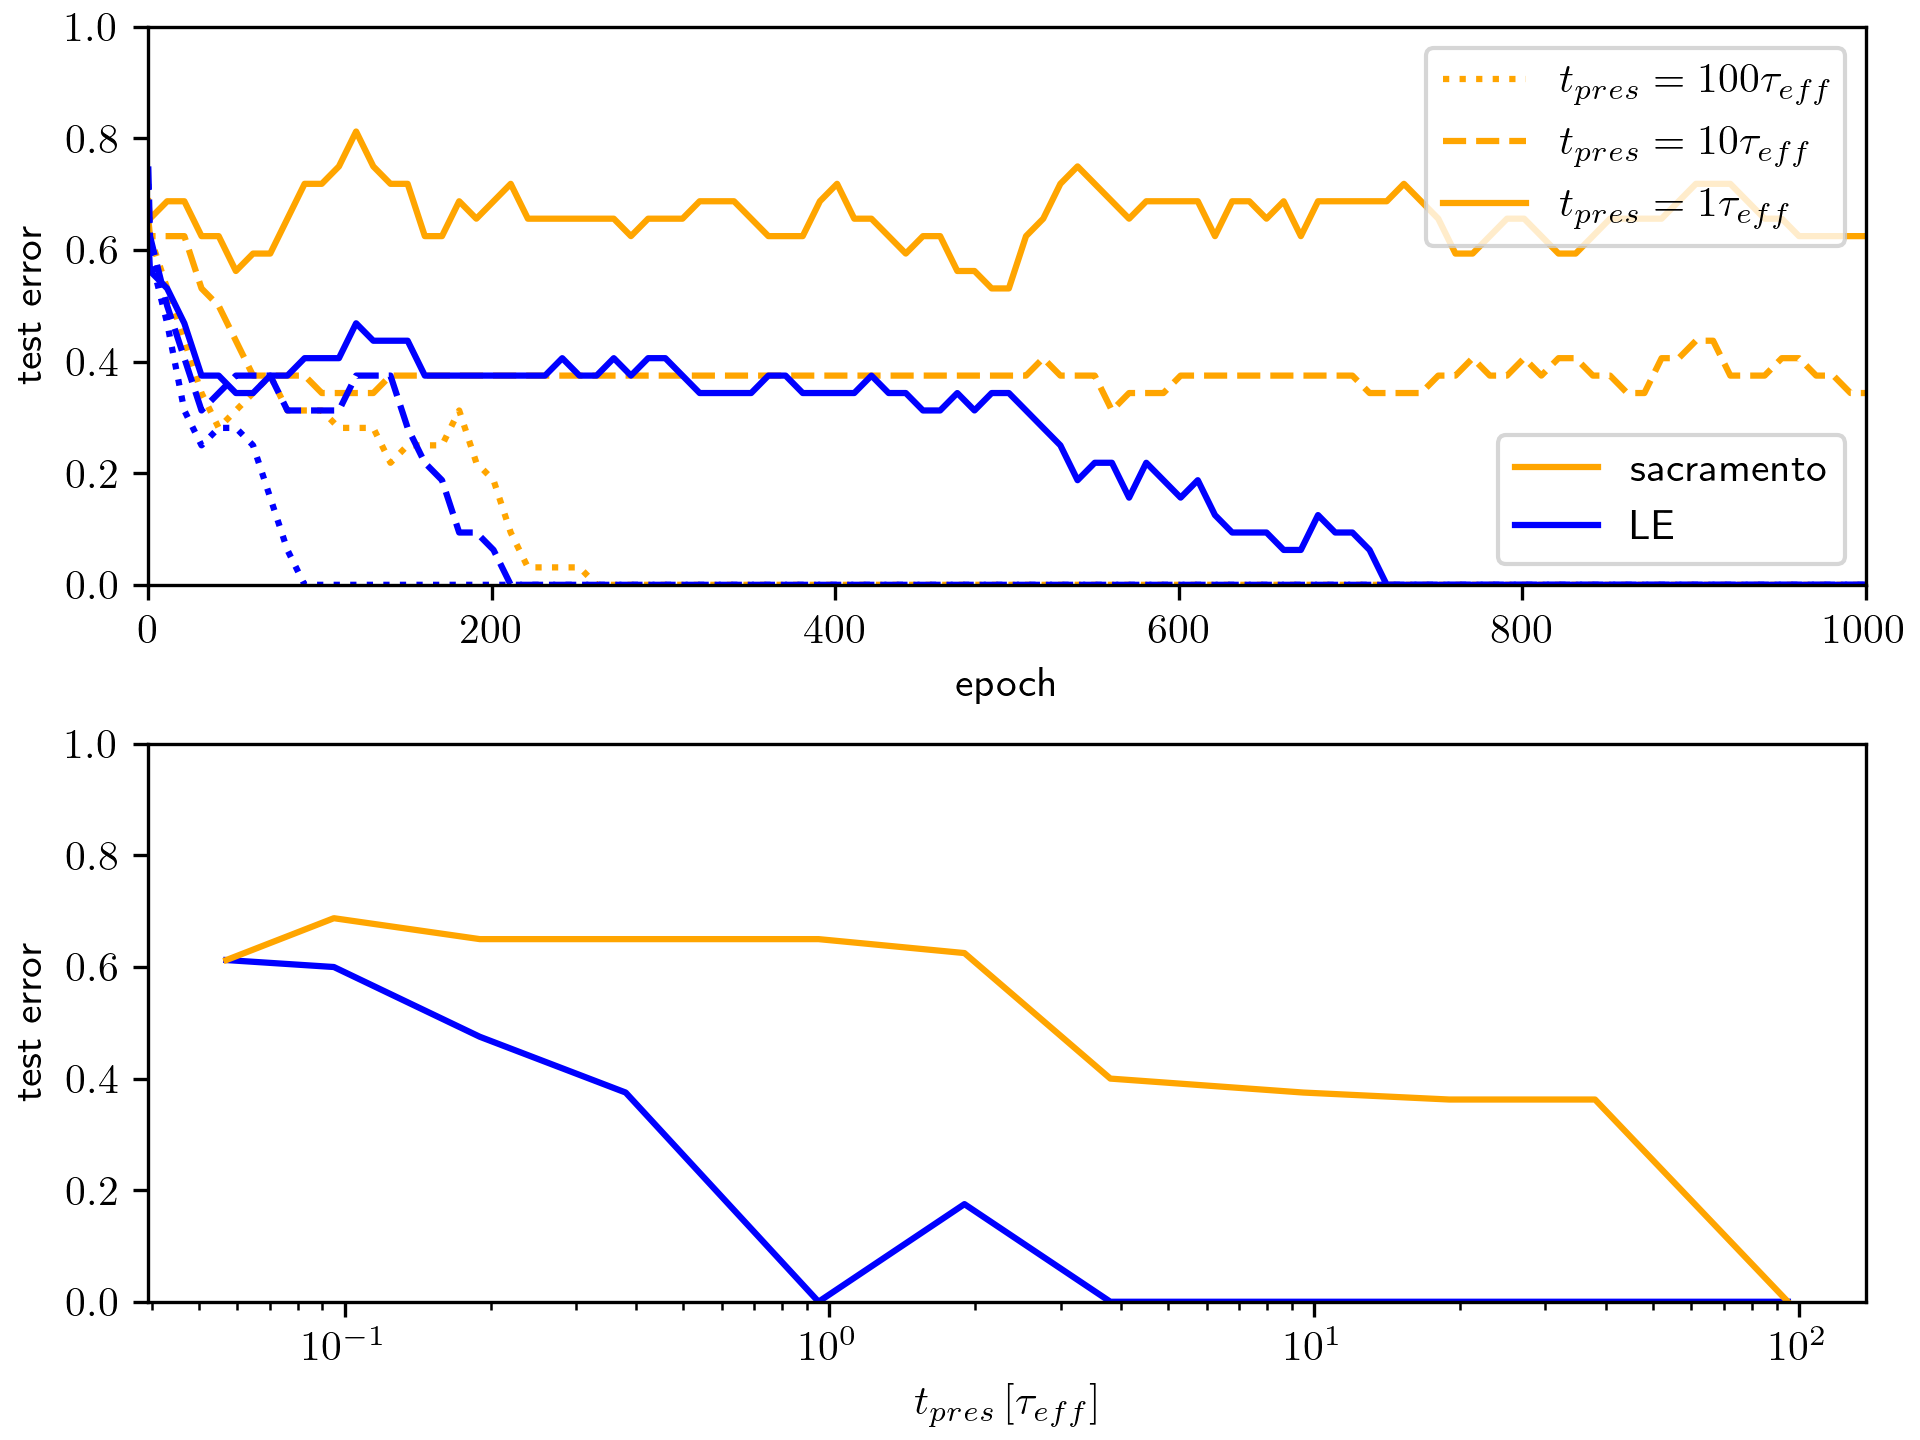
\includegraphics[width=0.9\textwidth]{fig_3_snest}
    \caption{Replication of Figure 3 from \cite{Haider2021} using networks of spiking neurons in the NEST simulator.
        \textbf{A:} Comparison between Original pyramidal microcircuit network by \cite{sacramento2018dendritic} and
        Latent equilibrium variant from \cite{Haider2021}. Shown is the training of a network with 9-30-3 neurons on the
        'Bars' Dataset from \todo{describe it} with three different stimulus presentation times. \textbf{B:} Test
        performance after 1000 Epochs as a function of stimulus presentation time.}
    \label{fig-bars-le-snest}
\end{figure}


\section{Separation of synaptic polarity}

A key limitation of the network model from \cite{sacramento2018dendritic} is the requirement that all synapses must be
able to assume both positive and negative polarities. When restricting any synaptic population in the network to just
one polarity, the network is unable to reach the self-predicting state \todo{expand?}. Thus, as the model is presented
here, activity in any neuron must be able to have both excitatory and inhibitory postsynaptic effects facilitated by
synaptic weights. This requirement is at odds with biology, which dictates a singular synaptic polarity for all outgoing
connections of a neuron, determined by neuron type and its corresponding neurotransmitter \citeme.


To investigate to what degree the plasticity rule can deal with this constraint, an experiment was conducted: An input
neuron population $A$  was connected to another population $C$ with plastic synapses that were constrained to positive
weights. In order to facilitate the required depression, $A$ was also connected to a population of inhibitory
interneurons $B$ through excitatory synapses with random and non-plastic weights. The interneurons in turn were
connected to $C$ through plastic, inhibitory connections arriving at the same dendrite. When inducing a dendritic error
in $C$, all plastic synapses in the network collaborated in order to minimize that error. When injecting a positive
basal error for example, the inhibitory weights ($C \rightarrow B$) decayed to 0, while excitatory synaptic weights ($A
\rightarrow B$) increased. Flipping the sign of that error injection had the opposite effect on weights, and likewise
compensated induced errors. This shows that a separation of synaptic polarity does not interfere with the principles of
the Urbanczik-Senn plasticity when depression is facilitated by interneurons.

Yet, as criticised by \citeme, the one-to-one connections between $A$ and $B$ are untypical for biological neural
networks \citeme. Hence, a second experiment was performed, in which $A$ and $B$ were fully connected through static
synapses with random positive weights. This added complexity did not hinder the error-correcting learning, as shown in
Figure \ref{fig-exc-inh-split}.


\begin{figure}[t]
    \centering
    \begin{minipage}{0.2\textwidth}
        \textbf{a)}\par\medskip
        \centering
        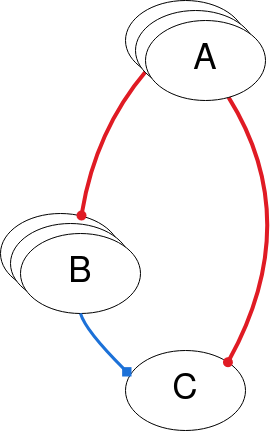
\includegraphics[width=0.9\textwidth]{fig_exc_inh_network}
    \end{minipage}\hfill
    \begin{minipage}{0.7\textwidth}
        \textbf{b)}\par\medskip
        \centering
        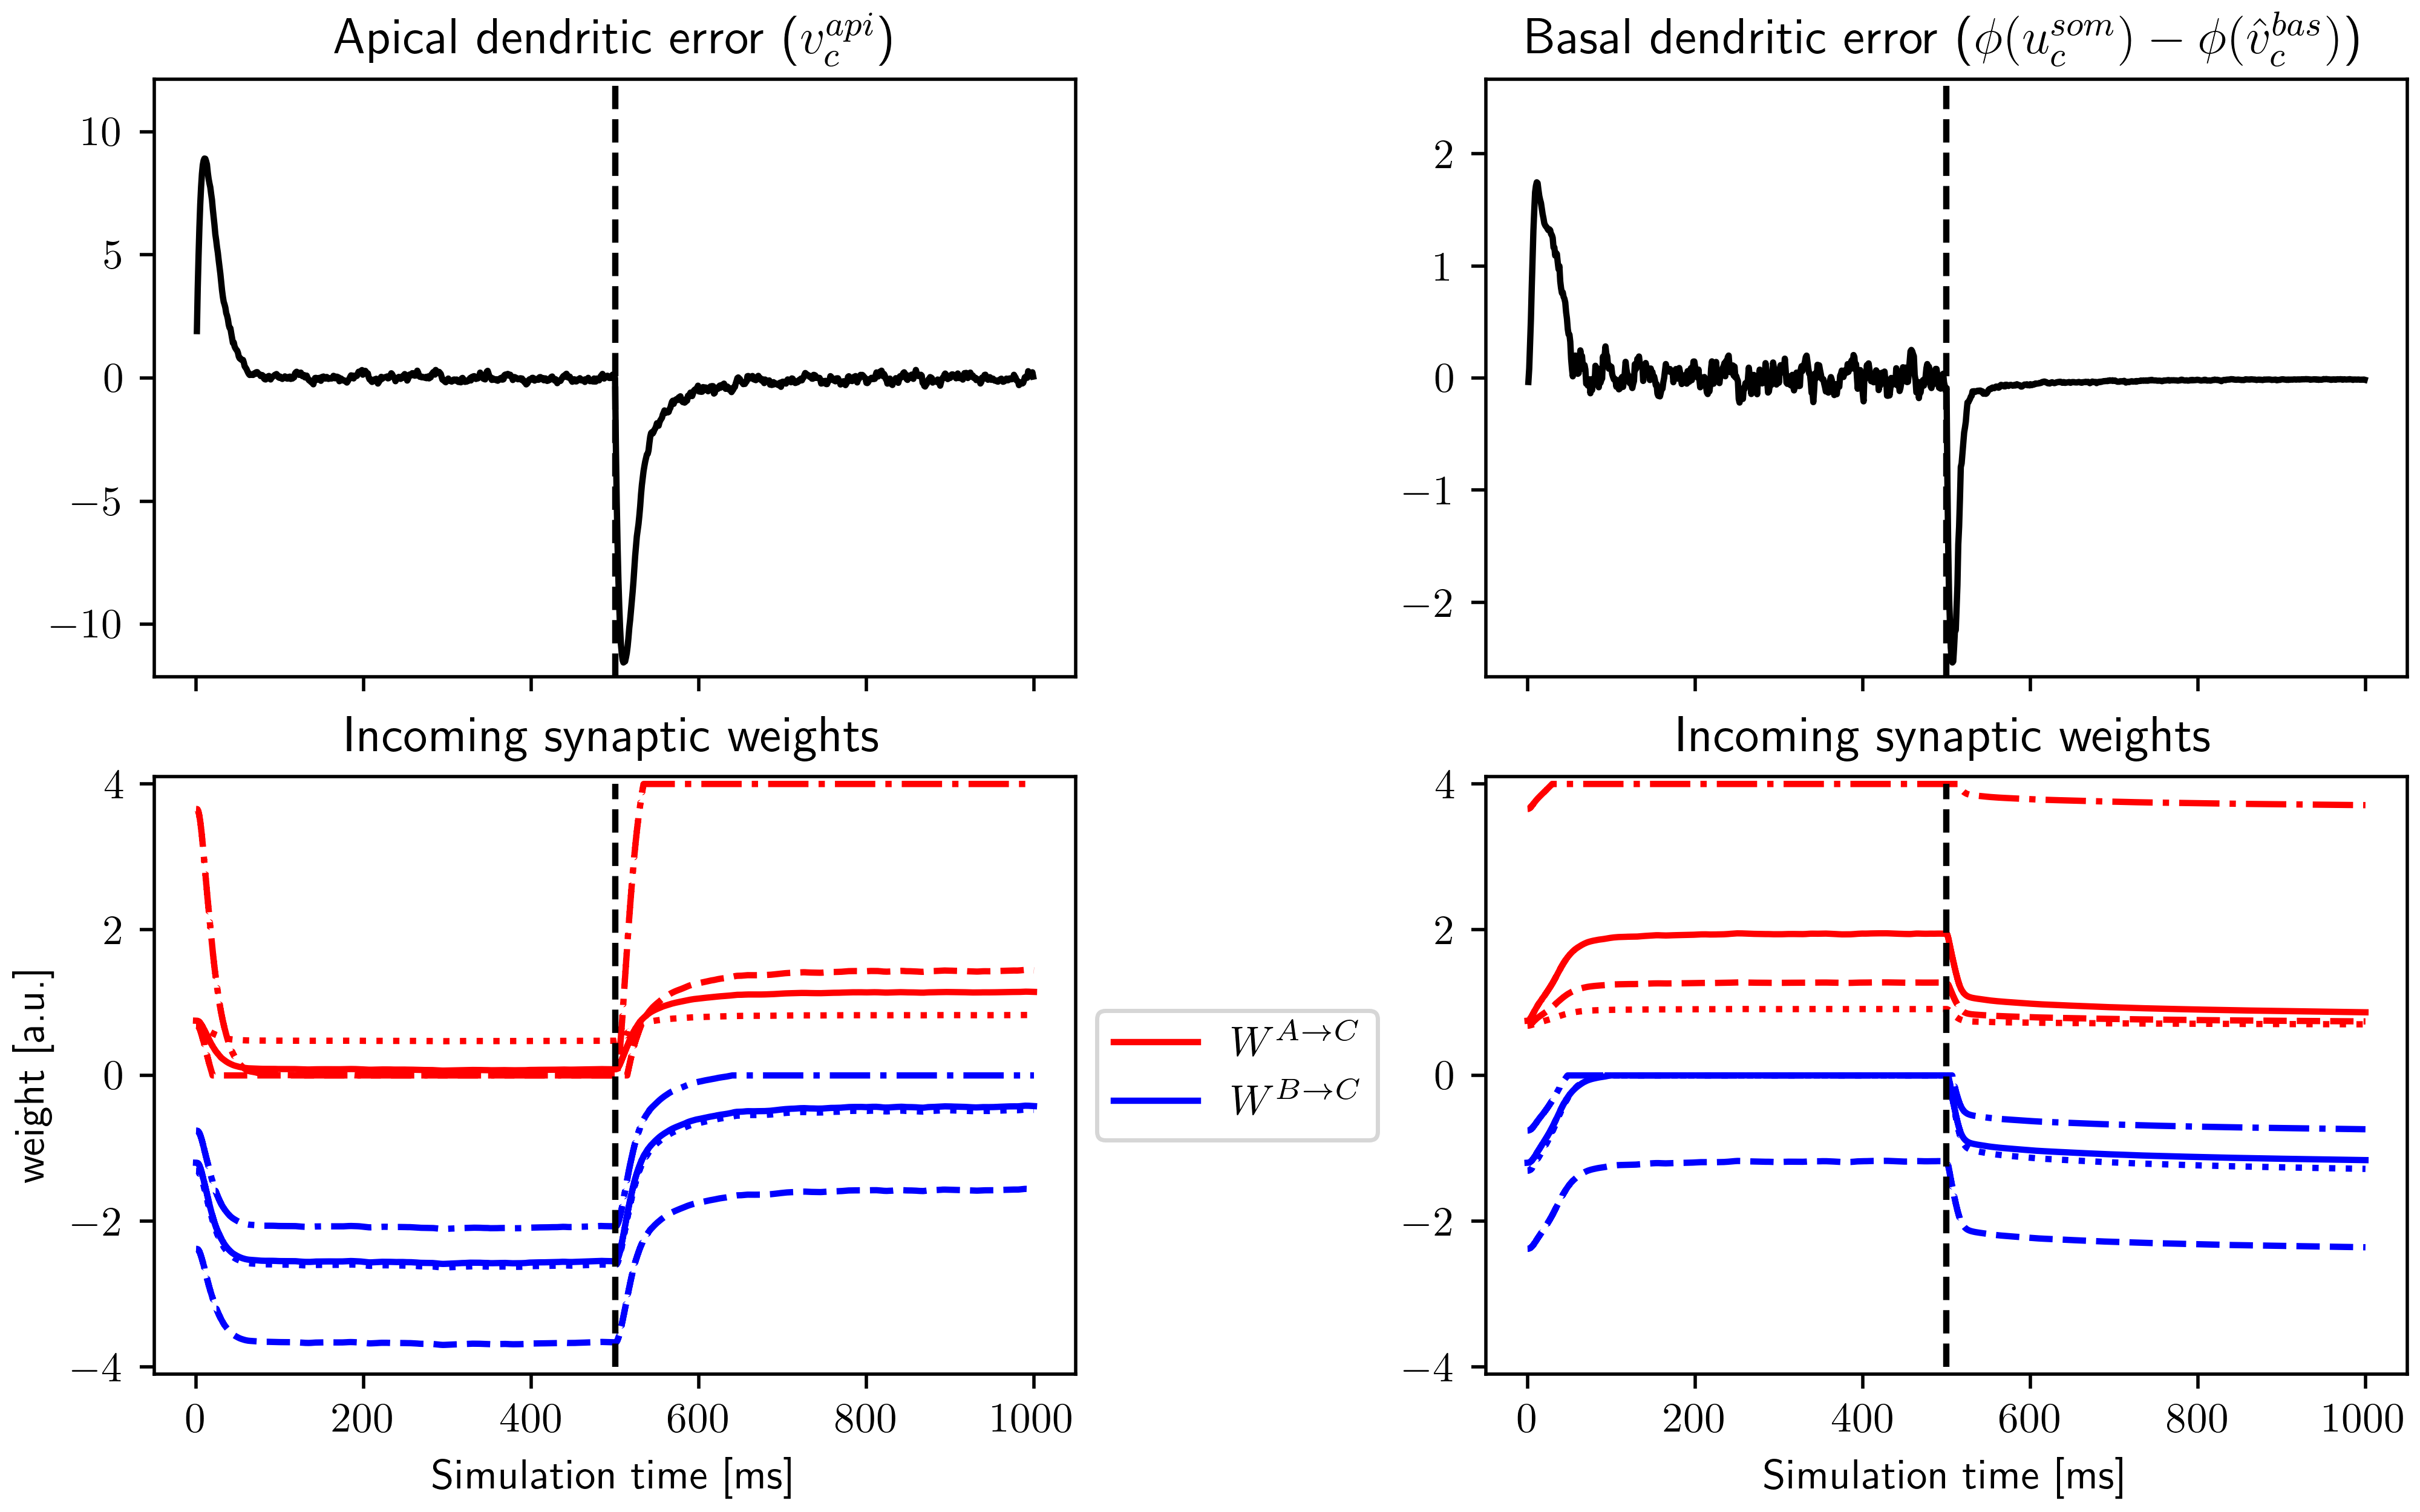
\includegraphics[width=0.9\textwidth]{fig_exc_inh_split}
    \end{minipage}
    \caption{Dendritic error minimization under biological constraints on synaptic polarity and network connectivity. 
    \textbf{a)} Network architecture. Excitatory population $A$ connects to a dendrite of Neuron $C$ both directly
    and through inhibitory interneuron population $B$. Only synapses $A\rightarrow C$ and $B \rightarrow C$ are plastic 
    through dendritic error rules. All connections between populations are 'all-to-all'\phrasing. \textbf{b)}
        \textit{Left:} All plastic synapses arrive at apical dendrites and evolve according to Equation
        \ref{eq-delta_w_pi}. \textit{Right:} Identical configuration regarding basal dendrites (Equations
        \ref{eq-delta_w_up},\ref{eq-delta_w_ip}). \textit{Top:} Dendritic error of a single target neuron. Errors of
        opposite signs are induced at $0$ and $500ms$ (vertical dashed line), and are quickly reduced
        through weight changes. \textit{Bottom:} Synaptic weights of incoming connections.}
    \label{fig-exc-inh-split}
\end{figure}

These results are useful, as they enable a biologically plausible way for excitatory long-range pyramidal projections to
connect to pyramidal neurons from another layer (i.e. in a different part of the cortex). The steps required to
facilitate this type of network are rather simple; A pyramidal neuron projection could enter a distant cortical area and
would only have to spread spread its axonal tree \phrasing within a layer that contains both pyramidal neuron dendrites 
and interneurons. If these interneurons themselves fully connect to the local pyramidal population, 



\section{Performance of the different implementations}

As stated in \cite{Haider2021}, simulating the present network with many neurons or more than one hidden layer quickly
becomes unfeasible when simulating the full leaky dynamics. To investigate how network size affects simulation time, all
three implementations created for this project were trained on the bars dataset for a single epoch with different
network sizes for a single epoch, in order to assess efficiency.


\begin{figure}[t]
    \centering
    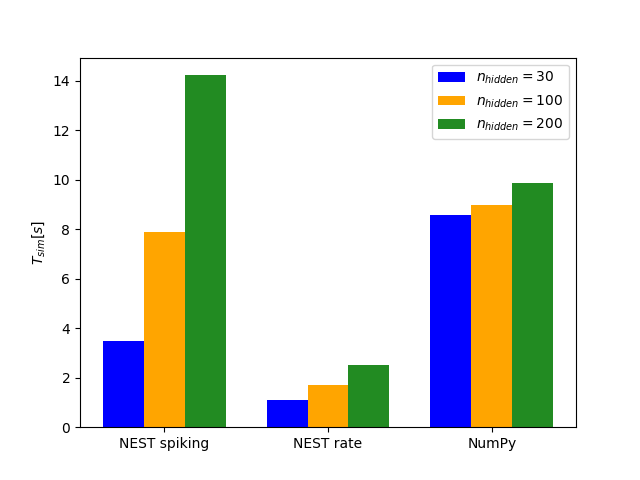
\includegraphics[width=0.8\textwidth]{fig_benchmark}
    \caption{Benchmark of the three different implementations using a network of $[9, n_{hidden}, 3]$ neurons per layer.
        $n_{hidden}=30$ was chosen as a baseline, as it is the default throughout all simulations on the Bars dataset.
        Networks were instantiated with the same synaptic weights and trained for a single epoch of 5 stimulus
        presentations of $100ms$ each. Simulations were performed on an \textit{AMD Ryzen Threadripper 2990WX} using 8
        cores for the NEST simulations at up to $3.0GHz$.}
    \label{fig-benchmark}
\end{figure}

The result of this comparison is shown in Figure \ref{fig-benchmark}. The NumPy network is slow at baseline, which is
likely explained by the fact that it is the only variant which is running on a single thread. This is due to a
limitation of NumPy, and could likely be improved greatly by using batched matrix multiplications, as are provided for
example by \texttt{PyTorch}\footnote{It is also possible, that the network code surrounding the NumPy computations is
    less efficient than the one for the NEST network. As this implementation was needed primarily to prove that neuron
    dynamics and synaptic updates were ported correctly to NEST, efficiency was a minor concern here and this was not
    investigated further.}.  Notably, this variant exhibits very little slowdown in response to an increase in network size.
My assumption is, that the vectorization of synaptic updates on a single thread scales up better than the communication
between threads that is required by most events in the NEST simulations. The NEST implementation using rate neurons
performed best in terms of speed across the board. This result was slightly surprising, as the demand on the
communication interface between threads is very high, since all neurons transmit an event to each of their postsynaptic
targets at every time step.

Finally, the novel spiking variant of this model performed substantially worse than anticipated. Particularly in
comparison to the rate implementation, I initially expected substantial performance improvements. The Difference between
the two was even greater when simulating on an office-grade processor (Benchmark was also run on an \textit{Intel Core
    i5-9300H} at $2.40GHz$, results not shown). Three hints about the comparatively poor performance can be deduced: For
one, both the rate and the spiking neuron model employ almost identical neuron models, with minor changes to
parametrization and output generation. Thus, updates to the neuron state are unlikely to be responsible for the worse
performance. Secondly, the number of Events transmitted between neurons is much lower for the SNN compared to

the \textit{relative} performance decrease when increasing the number neurons by the same amout is much greater for the
spiking network. Thus, the most likely cause of slowdown are the updates at the synapses. This is supported by the fact,
that the number of synapses increases much faster for this kind of network than the number of neurons. For the given
network of $n_{x} = 9$ input neurons, $n_y = 3$ output neurons and $n_{h}$ neurons in the hidden layer $l$, the number
of total synapses in the network is given by

\begin{align}
    n_{synapses} & = |w_{l}^{up}| + |w_{l}^{pi}| + |w_{l}^{ip}| + |w_{l}^{down}| + |w_{y}^{up}| \\
                 & = n_h n_x + n_h n_y + n_y n_h  + n_h n_y + n_y  n_h                          \\
                 & = n_h (n_x + n_y^4)
\end{align}

with $|w|$ of a weight matrix $w$ in this case denoting the total number of elements in that matrix \what{Is there a
    more conventional notation?}. Thus, the number of synapses in a network grows much faster than the number of total
neurons when increasing the size of the hidden layer.

availis given by the stark increase in






